\section{CrashSimulator Approach Details}

    \begin{figure*}[t]
        \center{}
        \fbox{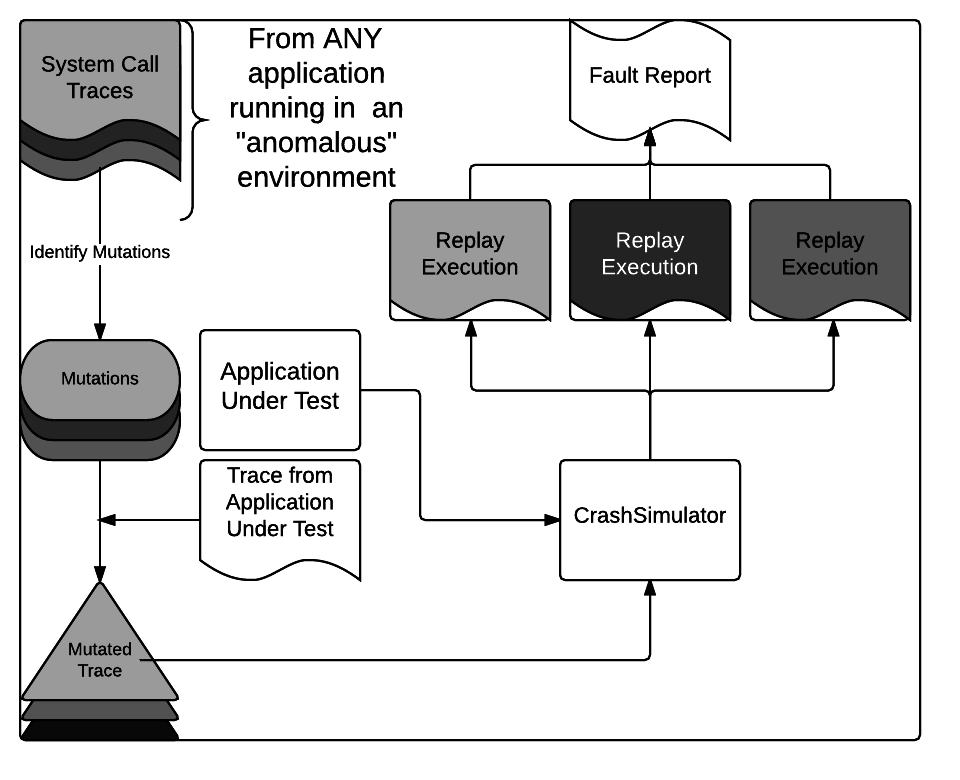
\includegraphics[scale=.5]{Architecture}}
        \caption{CrashSimulator Architecture: The process of gathering anomalous traces and the process of performing\\
        tests based on those traces are separate. Traces can be gathered ahead of time and used for testing later.\\
        Similarly, testing can performed repeatedly using the same set of traces. In this way, CrashSimulator can be\\
        used like a suite of unit tests.}

    \end{figure*}

    \subsection{Architecture}

        At a high level CrashSimulator is organized into three primary modules. The first module is responsible for
        interpreting the input system call traces and identifying opportunities to inject faults into the application
        under test. The second module's primary purpose is producing mutated versions of the input ``clean'' system call
        trace. The specific mutations it makes are based on the anomalies identified during analysis of the input system
        call traces. The final module is responsible for iterating through the set of anomalous system call traces in
        order to test each one of them. For each anomalous trace, this module launches a instance of the application
        under test and replays the anomalous system call trace. During this process, it monitors the application's
        behavior and reports any faults.

        For this implementation, the first module's duties are handled by NetCheck. CrashSimulator's architecture allows
        for one or more tools that can identify anomalies in a system call trace to fill this role assuming appropriate
        adapter code exists. This code must transform the output from the tool or tools performing the system call trace
        analysis into a format that can be inserted into CrashSimulator's anomaly store.

        All three primary CrashSimulator modules are packaged together and interact with each other at the appropriate
        times without user intervention. At this point, CrashSimulator itself is available as a virtual machine
        appliance compatible with the \emph{Virtual Box} virtual machine hosting software. The reasons for distributing
        CrashSimulator in this manner are threefold. First, this distribution method ensures that all of
        CrashSimulator's dependences are installed and configured appropriately. Second, this method provides an
        environment for taking system call traces that is known to be complete tool-wise and compatible with
        CrashSimulator. Finally, and most importantly, this method provides an environment that is known to be
        compatible with the details of CrashSimulator's system call replay techniques.

        CrashSimulator's source code is available and, while other environments may be untested, it should function
        correctly on any platforms that meet the criteria described above.

    \subsection{Anomaly Identification}

        The first step in CrashSimulator's operation is the analysis of the set of input system call traces recorded
        from other applications running in the intended deployment environment. These traces can be taken from any
        application that as environmental requirements that are reasonably similar to the application under test. For
        example, a web server could likely be effectively tested by CrashSimulator when CrashSimulator is given system
        call traces from other applications that make heavy use of the network. Testing a web browser with traces from
        an application that has no network usage at all would result in less effective testing.

        CrashSimulator was designed to accept identified anomalies from any tool that can output them in the proper
        format. In this implementation, CrashSimulator was written to accept the output of NetCheck. NetCheck readily
        able to identify a wide variety of anomalous behaviors related to network communication between one or more
        hosts. During normal operation, NetCheck analyzes a group of input system call traces and attempts to produce a
        diagnosis for network related faults. When operating as an anomaly identification tool for CrashSimulator its
        operation remains the same. Adapter code in CrashSimulator allows the normal output from NetCheck to be consumed
        without any modifications to NetCheck itself. This output is used to derive the mutations that will be made to
        the application under test's ``ideal'' system call trace in order to induce the faults NetCheck identified in
        the applications that yielded the input system call traces.

        This process of identifying anomalies does not need to be performed for each run of the test suite.
        CrashSimulator maintains a corpus of anomalies it has extracted from sample traces. These anomalies can be used
        to produce mutated traces for any future application that it tests. This allows a developer to build up a set of
        anomalies that were identified from each of their target environments. The developer can then test an
        application against this set of anomalies and get an idea of how their application will behave should it
        encounter the anomalies a deployment environment.

    \subsection{System Call Traces}

        Where other tools base their operation of direct analysis of the application under test CrashSimulator operates
        based on information gleaned from system call traces. This gives CrashSimulator several advantages over similar
        tools. First, CrashSimulator operates in a language independent manner. It can test any program given two
        conditions hold true:

        \begin{enumerate}
            \item{The application can run in the testing environment}
            \item{System call traces can be recorded from from applications similar to the application under test while
                they run in the intended deployment environment}
        \end{enumerate}

        Utilizing system call traces provides CrashSimulator with two advantages over similar tools. First,
        CrashSimulator has no need for complex language parsing and analysis code. It can test an application regardless
        of the programming language it was written in. Second, while other tools focus on the application under test in
        isolation, CrashSimulator is able to extensively test the interfaces between the application under test and its
        environment. This means that faults resultant from these interfaces are readily identified. For example,
        existing tools are able to quickly test for flaws that result from improper parsing of data once it
        has been received from across a network. CrashSimulator is able to induce and identify flaws that result from
        improper behavior during the network communication itself. This second type of flaw is much more difficult to
        identify replicating the application's intended deployment environment or deploying the application and testing
        it live.
